\documentclass[12pt,a4paper]{article}
\usepackage[english,italian]{babel}%lingua
\usepackage[margin=2cm]{geometry} %margini
\usepackage{float} %float per immagini e tabelle
\usepackage{graphicx} %figure
\usepackage{longtable} %tabelle
\newcommand\crule[3][black]{\textcolor{#1}{\rule{#2}{#3}}}
\usepackage[table]{xcolor} %colori tabelle
\usepackage{lastpage} %numero pagine
\usepackage{fancyhdr} %stile template
\usepackage{hyperref} %stile template
\usepackage{xurl} %url a capo
\usepackage{textcomp} %elenchi puntati carini
%Colori definiti
\definecolor{green}{HTML}{0a6b2a}
\definecolor{grey}{HTML}{cccccc}
%Righe per il template
\pagestyle{fancy}
\fancyhf{} %eliminare le cose già presenti nella pagina (numero)
\rhead{\textbf{\leftmark}}
\lfoot{\textit{La Tana del Luppolo}}
\rfoot{\thepage\ / \pageref{LastPage}}
\renewcommand{\footrulewidth}{1pt}
\renewcommand{\headrulewidth}{1pt}


\title{Progetto di Tecnologie Web}
\author{}
\date{Anno accademico 2020/2021}
\begin{document}
\pagenumbering{gobble}
\maketitle
\begin{figure}[H]
	\centering
	
\includegraphics[width=8cm]{utility/logo.png}
\end{figure}
\begin{table}[H]
	\centering
	\renewcommand{\arraystretch}{2}
	\rowcolors{2}{grey}{white}
	\begin{longtable}{c c c}
		\rowcolor{green}\multicolumn{3}{c }{\textcolor{white}{\textbf{Componenti}}}\\
		\endhead
		 Ayoub & Maher & 1187406 \\
		 Denisa & Hida & 1204284 \\
		 Giacomo & Sassaro & 1187566 \\
		 Gianpiero Giuseppe & Tovo & 1193350 \\
	\end{longtable}
\end{table}

\begin{center}
	\textbf{Indirizzo sito web}: http://tecweb.studenti.math.unipd.it/gsassaro\\
	\textbf{Email referente del gruppo}: giacomo.sassaro@studenti.unipd.it
\end{center}

\begin{table}[H]
	\centering
	\renewcommand{\arraystretch}{2}
	\rowcolors{2}{grey}{white}
	\begin{longtable}{c | c c}
		\rowcolor{green}\textcolor{white}{\textbf{Utenti}} & \textcolor{white}{\textbf{Username}} & \textcolor{white}{\textbf{Password}}\\
		\endhead
		Admin & admin & admin\\
		User & user  & user \\
	\end{longtable}
\end{table}
\newpage
\pagenumbering{arabic}
\tableofcontents
\newpage
\section{Introduzione}
\subsection{Abstract}
\textit{La Tana del Luppolo} è un sito che nasce come vetrina per un piccolo birrificio artigianale. L'idea é quella che i clienti possano lasciare delle recensioni e dare dei voti alle birre che assaggiano, ed eventualmente acquistano durante le degustazioni organizzate periodicamente dall'azienda.
\subsection{Analisi dell'utenza}
Il sito web si rivolge ad un utenza molto variegata, prevalentemente persone appassionate di birra o alla ricerca di nuove passioni. Tale utenza comprende dai più giovani, molto abili e intuitivi nella navigazione, fino agli utenti più anziani, in genere con meno dimestichezza nel navigare su internet.

\subsection{Funzionalità}
Per accedere al sito, data la natura dei contenuti, viene predisposta una pagina utile ad assicurarsi che gli utenti siano maggiorenni e ad impedire quindi di proseguire in caso contrario. Superata la verifica dell'età viene quindi visualizzata una vetrina di birre consigliate e l'utente può procedere richiedendone dei dettagli più approfonditi, visualizzando la lista completa delle birre disponibili, accedendo al sito oppure visualizzando i contatti dell'azienda.
La registrazione al sito permette di aggiungere e rimuovere recensioni personali delle birre, composte da una descrizione e da un voto in decimi.
Gli account amministratori, oltre a gestire le proprie recensioni, hanno la possibilità di rimuovere tutte le recensioni in modo da poter svolgere la loro funzione di moderazione.
Gli account possono essere elevati al ruolo di admin dagli amministratori del database, che si occupano inoltre dell'inserimento di nuove birre.


\newpage
\section{Progettazione}
E' stata scelta una strategia di progettazione \textit{Responsive Web Design}, il sito infatti é in grado di adattarsi graficamente in modo automatico in base al dispositivo con il quale viene visualizzato. \\
Si è preferito usare  XHTML5  perché  ci  permette  di  usare  la  specifica  WAI-ARIA, discussa in seguito.\\
Il progetto è stato affrontato con un approccio top-down, individuando elementi generici da implementare e procedendo quindi con lo sviluppo di pagine e funzioni.

\subsection{Struttura delle pagine}
Sono di seguito riportati i differenti elementi della struttura delle pagine del sito.
\paragraph{Header}
L' header contiene il logo ed il nome del sito, un pulsante per visualizzare la barra di ricerca, un pulsante per accedere al profilo personale ed una barra di navigazione con i riferimenti alle principali pagine del sito.\\
\'E presente in tutte le pagine del sito.
\paragraph{Breadcrumb}
Sotto alla testata è situata la breadcrumb, che permette all'utente di orientarsi visualizzando il percorso dalla homepage fino alla pagina corrente.\\
La breadcrumb non è visibile nelle pagine di avviso di contenuto non trovato, di accesso negato e di conferma dell'eliminazione dell'account.
\paragraph{Main}
La sezione Main visualizza il contenuto principale e caratterizzante della pagina.
\paragraph{Footer}
Al piede della pagina è situato il footer che riporta informazioni sul progetto e i relativi certificati di validazione.\\
\'E presente in tutte le pagine del sito.

\subsection{Struttura del sito}
L'index page del sito reindirizza alla pagina di verifica dell'età, mentre conduce direttamente alla homepage se nelle variabili di sessione è indicato che l'utente ha già eseguito la verifica ed è maggiorenne.\\
La verifica viene eseguita dalla pagina \textit{ageverification} stessa ed ogni altra pagina reindirizza a quest'ultima se rileva che nella sessione dell'utente non è presente la variabile che rappresenta l'avvenuta verifica.\\
Di seguito si riportano le pagine del sito e le rispettive caratteristiche.

\paragraph{Home}
L'\textit{homepage} è la pagina che viene mostrata all'utente dopo la verifica dell'età e contiene una lista di birre in offerta o consigliate dall'azienda.

\paragraph{Prodotti}
La pagina \textit{prodotti} visualizza tutte le birre disponibili nel database, suddivise in pagine.\\
La pagina viene inoltre utilizzata per visualizzare i risultati di una ricerca tramite la barra di ricerca.

\paragraph{Dettagli}
La pagina \textit{dettagli} visualizza informazioni complete e recensioni della birra scelta dalla pagina \textit{prodotti}.\\
Se l'utente ha effettuato l'accesso vengono visualizzati i controlli per aggiungere e rimuovere recensioni.

\paragraph{Contatti}
La pagina \textit{contatti} contiene una breve descrizione dell'azienda ed il contatto telefonico e di posta elettronica dell'azienda.

\paragraph{Spazio utente}
La registrazione e l'accesso degli utenti viene gestita dalle pagine \textit{login} e \textit{registrazione} mentre \textit{dettagliaccount} e \textit{modificadati} permettono la visualizzazione e la modifica dei dati del proprio profilo.

\paragraph{Avvisi}
Il tentativo di accesso ad aree vietate o a contenuti non disponibili viene notificato dalle pagine \textit{accessdenied} e \textit{notfound} mentre il risultato di query viene visualizzato in sezioni della pagina dalla quale viene eseguita l'operazione.\\
La pagina \textit{deleteaccount} avverte della corretta eliminazione dell'account e la pagina \textit{logout} si occupa di terminare la sessione e reindirizzare l'utente alla homepage.

\subsection{Attori}
Vengono di seguito elencati i possibili tipi di utenti che possono interagire con il sito.
\begin{itemize}
\item \textbf{Utente non abilitato:} Se l'utente non ha una sessione attiva o ha dichiarato di essere minorenne, ogni tentativo di accesso alle pagine del sito risulta in una ridirezione alla pagina di verifica dell'età, dalla quale può proseguire solo dopo aver confermato di essere maggiorenne;
\item \textbf{Utente maggiorenne e non loggato:} Un utente che ha dichiarato di essere maggiorenne e non è loggato nel sito ha accesso a tutte le pagine tranne quelle di gestione dell'account; il tentativo di accesso a quest'ultime verrà negato e segnalato da una pagina apposita.
L'utente può accedere alla pagina di registrazione attraverso il link \textit{Registrati} nella pagina login, raggiungibile dal tasto account situato nell'header.
Nelle pagine di dettagli delle birre saranno visualizzate le recensioni ma non ci sarà la possibilità di modificarle o aggiungerne di nuove;
\item \textbf{Utente maggiorenne e loggato:} Gli utenti che hanno effettuato l'accesso possono visitare tutte le pagine del sito ed hanno la possibilità di aggiungere ed eliminare le proprie recensioni.
Dalla pagina \textit{account} possono inoltre visualizzare e modificare i propri dati, effettuare il logout o eliminare l'account;
\item \textbf{Utente amministratore:} Un utente amministratore ha accesso a tutte le pagine del sito ed ha la possibilità di eliminare anche le recensioni degli altri utenti.
Un account deve essere eletto amministratore dagli operatori del database.
\end{itemize}

\newpage
\subsection{Accessibilità}
Seguendo le linee guida per l'accessibilità del contenuto Web (WCAG 2.1), abbiamo modificato e aggiunto specifici elementi per rendere il nostro sito accessibile a tutti i nostri utenti, tra cui anche quelli che usano tecnologie assistive.   
\subsubsection{Percepibile}
\paragraph{Alternative testuali}
Tutti i contenuti non testuali presentati all'utente hanno un'alternativa testuale equivalente.
\paragraph{Adattabile}
Per la strategia seguita (\textit{Responsive Web Design} il sito non perde informazioni o struttura quando viene visualizzato in dispositivi diversi.
\paragraph{Distinguibile}
L'uso dei colori non è stato fatto solamente per presentazione ma si usano colori specifici che rappresentano emozioni, come per esempio l'uso del verde quando un'azione esegue con successo e l'uso del rosso quando succede il contrario.
La rappresentazione visiva del testo e immagini contenenti testo ha un rapporto di contrasto di almeno 7:1, che ci fa superare il test WCAG AAA.
\subsubsection{Utilizzabile}
I controlli sono correttamente assegnati ad una label e all'interno di form sono raggruppati da un tag \textit{fieldset}, descritto da un rispettivo tag \textit{legend}.\\
Tramite l'attributo \textit{tabindex} l'ordine di focus tramite tasto tab viene corretto o nascosto ad alcuni elementi di presentazione, come ad esempio le icone degli utenti delle recensioni, che sono quindi marcate con il valore \textit{presentation} dell'attributo \textit{role}.\\
I tag di heading sono stati utilizzati seguendo una corretta gerarchia ed in modo coerente per segnalare titoli e contenuti delle sezioni.\\
Nel sito sono assenti link circolari e sono presenti un \textit{hidden link} utile allo screen reader per saltare al contenuto della pagina ed un \textit{back-to-top-button} per tornare all'inizio della pagina.\\
\subsubsection{Comprensibile}
In aiuto ai sistemi di screen-reading sono inoltre segnalate le parole inglesi dagli attributi \textit{xml:lang} e \textit{lang}, le immagini principali sono dotate di un attributo \textit{alternative text} consono e i alcuni controlli marcati con l'attributo \textit{aria-label}.\\
I valori provenienti dai controlli, prima di essere processati lato server vengono validati e sanitizzati.
\subsubsection{Robusto}
Tutti i tag sono chiusi in modo corretto ed ogni pagina è caratterizzata da una lista adeguata di keyword.
\newpage
\subsection{Database}
Il sito sfrutta un database molto semplice, composto da tre tabelle:
\begin{itemize}
\item \textbf{Utenti:} raccoglie i dati anagrafici e di accesso di tutti gli utenti registrati al sito. \'E stata implementato un campo \textit{admin\textunderscore flag} che viene posto a \textit{TRUE} nel caso in cui l'account sia amministratore; la chiave primaria é un id auto-incrementate e \textit{username} é chiave univoca, così da impedire la registrazione al sito di più utenti con lo stesso username. Abbiamo deciso di non memorizzare la data di nascita nel database in quanto un utente che visita il sito deve aver dichiarato precedentemente di essere maggiorenne, un campo \textit{data\textunderscore nascita} per gli utenti non verrebbe quindi utilizzato e risulterebbe superfluo;
\item \textbf{Birre:} raccoglie i dati delle birre presenti nel sito. La chiave primaria é un id auto-incrementante, mentre il nome é chiave univoca, così da impedire l'inserimento di più birre con lo stesso nome;
\item \textbf{Recensioni:} raccoglie le recensioni delle birre (testo e voto) lasciate dagli utenti. La chiave primaria é un id auto-incrementante, ed essendo l'unica chiave un utente può lasciare più recensioni della stessa birra. Il campo \textit{utente} é chiave esterna riferita al campo \textit{id} della tabella \textit{Utenti} mentre il campo \textit{birra} é la chiave esterna riferita al campo \textit{id} della tabella \textit{Birre}.
\end{itemize}
Il database é normalizzato.
\begin{figure}[H]
	\centering
	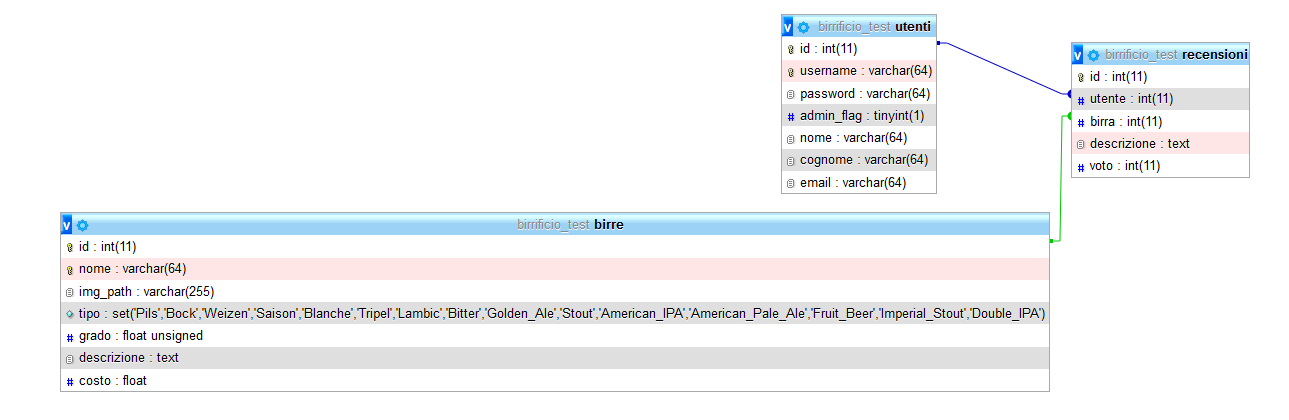
\includegraphics[width=16cm]{utility/db.png}
	\caption{UML database}
\end{figure}



\newpage
\section{Realizzazione}
Ogni pagina ha un suo scheletro in un file HTML, il quale viene aperto dal file \textit{nome\textunderscore pagina.php} tramite la funzione \textit{file\textunderscore get\textunderscore contents()}, successivamente la pagina viene popolata dalla classe PHP \textbf{htmlMaker} da noi sviluppata e solo a questo punto viene mostrata all'utente.\\
Così facendo riusciamo a tenere totalmente separato il comportamento dalla struttura, riusciamo a gestire le sessioni e non abbiamo bisogno di fare chiamate AJAX dalle pagine.
\subsection{HTML}
Abbiamo cominciato scrivendo un header e un footer che fossero unici per tutte le pagine, questi due file HTML vengono letti dalla classe \textit{htmlMaker} e inseriti in tutte le pagine presenti nel sito. Successivamente abbiamo iniziato a scrivere il codice HTML di ogni altra pagina, a partire dalla home, prodotti e contatti. Man mano che le pagine prendevano forma andavamo a spostare il codice HTML scritto, nella classe PHP responsabile della generazione del contenuto delle varie pagine.
\subsection{CSS}
Riguardo allo stile CSS, abbiamo lavorato parallelamente allo sviluppo delle pagine, a partire dallo stile principale condiviso per poi procedere anche con lo stile per dispositivi mobile, la quale presentazione è gestita da un apposito foglio di stile che ottimizza la visualizzazione e dispone barra di navigazione e pulsanti di ricerca e account nel menu ad hamburger nella parte destra dell'header.


\begin{figure}[H]
	\centering
	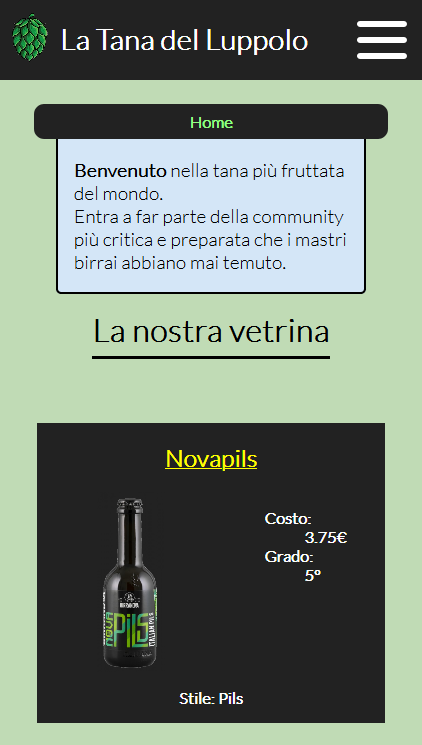
\includegraphics[width=6cm]{utility/home_mobile.png}
	\caption{Il layout mobile della homepage}
\end{figure}

\pagebreak

Infine è stato predisposto un foglio di stile per la stampa dalla quale sono stati nascosti alcuni elementi giudicati superflui (ad esempio la barra di navigazione o i pulsanti back-to-top-button, ricerca e account) o modificati per migliorarne la presentazione (come la breadcrumb, le recensioni o la grandezza delle immagini principali).

\begin{figure}[H]
	\centering
	\caption{Il layout di stampa della pagina Prodotti}
	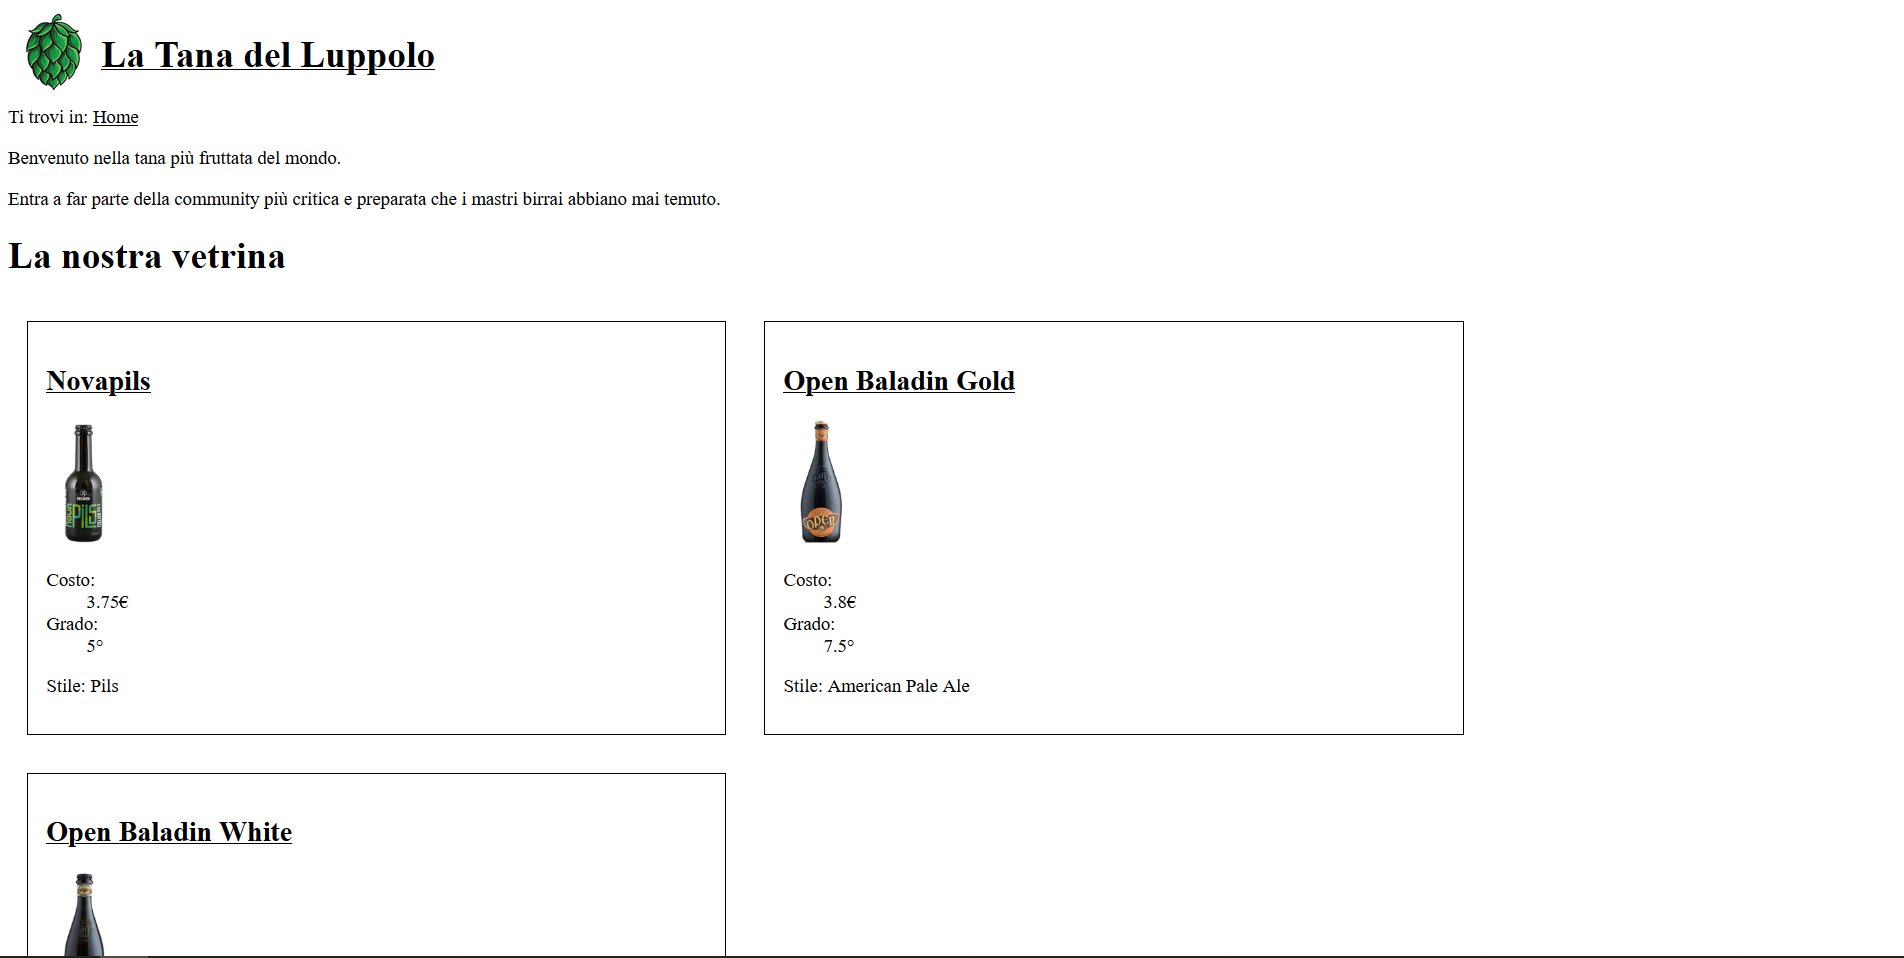
\includegraphics[width=16cm]{utility/prodotti_printcss.png}
\end{figure}

I colori dominanti del sito sono il grigio scuro e un verde pistacchio per header, sfondi ed altri elementi di presentazione mentre vengono utilizzati il nero, il verde ed il giallo per testi e link.\\

% palette colori
Sfondi ed elementi
\definecolor{hdgray}{RGB}{34, 34, 34}
\definecolor{pistacho}{RGB}{192, 219, 181}
\definecolor{puffo}{RGB}{212, 230, 247}
\crule[hdgray]{1cm}{1cm} \crule[pistacho]{1cm}{1cm} \crule[puffo]{1cm}{1cm} 


Testi e link
\definecolor{bcgreen}{RGB}{167, 255, 131}
\definecolor{hdgreen}{RGB}{216, 251, 216}
\crule{1cm}{1cm} \crule[yellow]{1cm}{1cm} \crule[bcgreen]{1cm}{1cm} \crule[hdgreen]{1cm}{1cm}
\\

La palette è stata scelta in modo da garantire una corretta visualizzazione anche da persone affette da diversi tipi di cecità o sensibilità del contrasto ed il contenuto del sito rimane correttamente visualizzabile anche senza il caricamento dello stile CSS.

\begin{figure}[H]
	\centering
	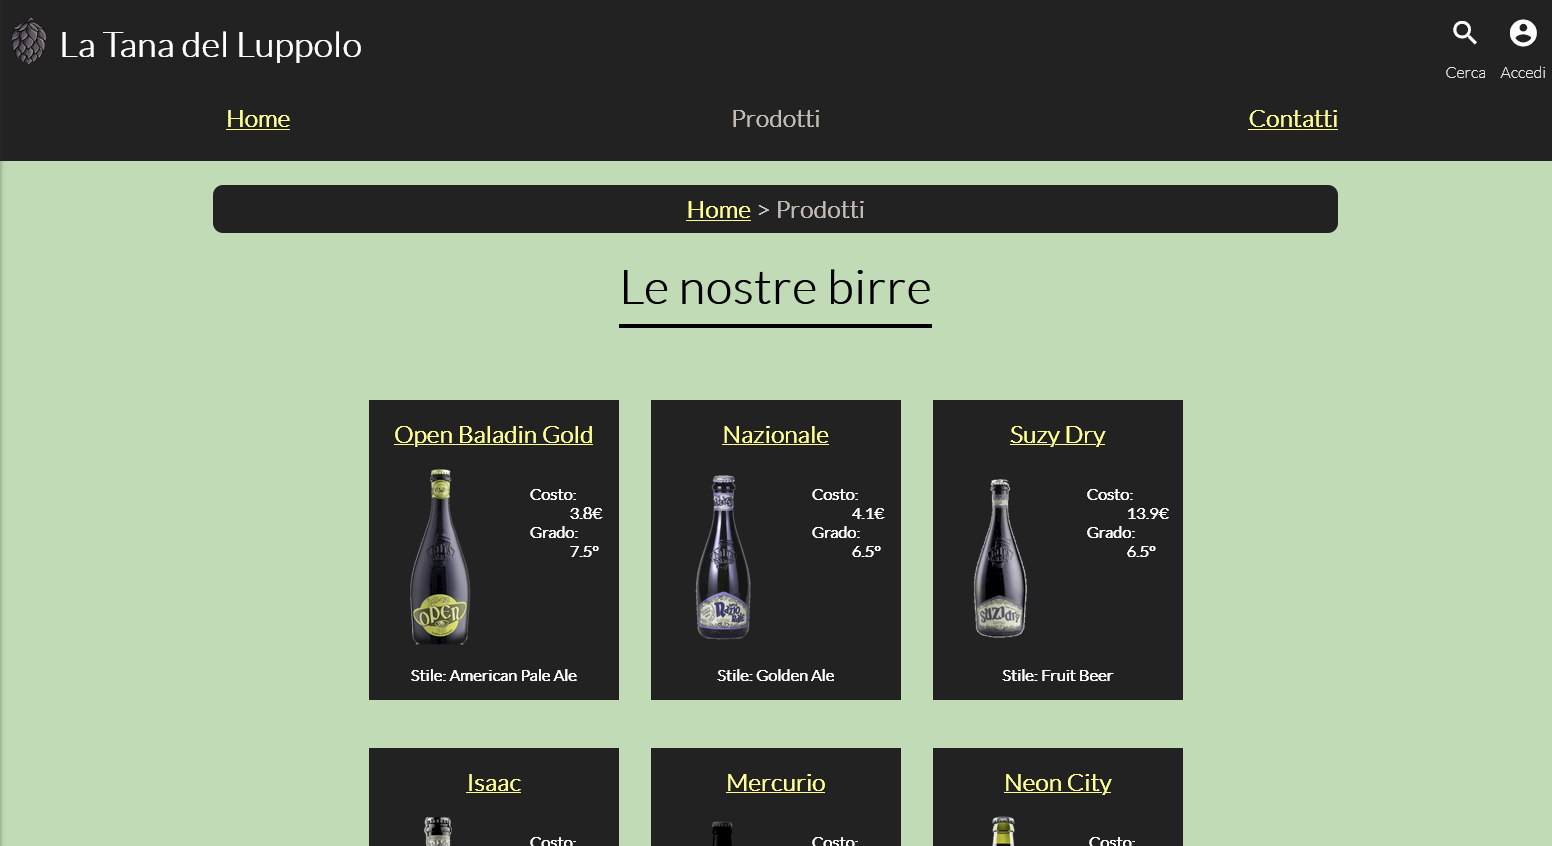
\includegraphics[width=16cm]{utility/prodotti_deuteranopia.png}
	\caption{Vista della pagina Prodotti da persone affette da deuteranopia (cecità al verde)}
\end{figure}


\subsection{Javascript}
\subsection{PHP}
Nel nostro sito, ogni pagina ha un suo file PHP, inoltre abbiamo creato due classi con metodi statici, così da non dover istanziare oggetti per richiamarne le funzioni:
\begin{itemize}
\item \textbf{htmlMaker.php:}
\item \textbf{dbConnection.php:}
\end{itemize}
\newpage
\section{Validazioni}


% ff extention WCAG Color Checker https://addons.mozilla.org/it/firefox/addon/wcag-contrast-checker
\subsection{WCAG Color Checker}
L'estensione\ap{1} per il browser Firefox non rileva problemi tra i colori scelti ed i livelli di contrasto.

% ff extention WAVE Evaluation Tool https://addons.mozilla.org/it/firefox/addon/wave-accessibility-tool/
\subsection{WebAIM WAVE Tool}
L'estensione\ap{2} per il browser Firefox non segnala problemi e valuta positivamente l'utilizzo dei tag, gerarchia degli heading e label dei controlli.

\subsection{Total Validator}
Tutte la pagine del sito sono state alidate attraverso l'estensione per browser di Total Validator\ap{4} e Total Validator Test\ap{3}. Il codice sorgente generato da PHP di ogni pagina è stato validato con standard \textit{XHTML5}, cosí da poter utilizzare i tag piú recenti forniti da HTML5, mantenendo una struttura in stile XHTML. Inoltre è stato verificato che le pagine garantiscano un'accessibilitá conforme agli standard \textit{WCAG21 AAA}.
\subsection{ChromeVox}
È stata usata l'estensione ChromeVox\ap{5} di Google Chrome per testare il funzionamento dello screen reader sul sito. ChromeVox interpreta le pagine come gli altri screen reader ed è facile da usare per i sviluppatori ed ovviamente da chi ne ha bisogno. Con l'uso di questo tipo di screenreader si è verificato che tutte le funzionalità del contenuto di una pagina sono utilizzabili tramite un'interfaccia di tastiera senza richiedere tempi specifici per la pressione dei singoli tasti.


\vfill
\section*{Links}
\begin{enumerate}
	\item WCAG Color Checker \url{https://addons.mozilla.org/it/firefox/addon/wcag-contrast-checker} 
    \item WebAIM WAVE Tool \url{https://addons.mozilla.org/it/firefox/addon/wave-accessibility-tool/} 
    \item Total Validator Test \url{https://www.totalvalidator.com/products/index.html}
    \item Total Validator Extension \url{https://www.totalvalidator.com/products/extension.html}
    \item ChromeVox \url{https://chrome.google.com/webstore/detail/screen-reader/kgejglhpjiefppelpmljglcjbhoiplfn}
\end{enumerate}
    
\newpage
\section{Organizzazione del lavoro}
Il lavoro tra i membri del gruppo é stato ripartito nel seguente modo:
\begin{itemize}
	\item \textbf{Ayoub Maher}:
	\begin{itemize}
		\item Lavoro sui file HTML;
		\item Creazione e maggioranza del lavoro sul file JS;
		\item Lavoro sui file CSS(css mobile);
		\item Lavoro sui file PHP;
		\item Stesura di alcune parti della relazione.
	\end{itemize}
	
	\item \textbf{Denisa Hida}:
	\begin{itemize}
		\item Lavoro sui file HTML;
		\item Lavoro sul file JS;
		\item Lavoro sui file CSS;
		\item Lavoro sui file PHP;
		\item Controllo con screenreader;
		\item Stesura di alcune parti della relazione.
	\end{itemize}
	
	\item \textbf{Giacomo Sassaro}:
	\begin{itemize}
		\item Lavoro sul file JS;
		\item Lavoro sui file CSS;
		\item Creazione e maggioranza del lavoro sui file PHP;
		\item Validazione del codice;
		\item Creazione e stesura di alcune parti della relazione.
	\end{itemize}
	
	\item \textbf{Gianpiero Giuseppe Tovo}:
	\begin{itemize}
		\item Creazione e maggioranza del lavoro sui file HTML;
		\item Lavoro sui file CSS;
		\item Lavoro sui file PHP;
		\item Controlli sull'accessibilità;
		\item Stesura di alcune parti della relazione.
	\end{itemize}
	
\end{itemize}

\newpage
\section{Note per l'utilizzo e l'installazione}
\subsection{Installazione}
I requisiti minimi per il corretto funzionamento del sito sono:
\begin{itemize}
\item \textbf{Server HTTP}, si consiglia APACHE;
\item \textbf{PHP versione 7.0 o superiore};
\item \textbf{DBMS compatibile}, si consiglia MariaDB;
\end{itemize}
\subsection{Credenziali}
Come riportato nella tabella ad inizio pagina le credenziali per l'accesso al sito sono:
\begin{itemize}
\item \textbf{Amministratore}:
	\begin{itemize}
		\item Username: admin;
		\item Password: admin.
	\end{itemize}

\item \textbf{Utente}:
	\begin{itemize}
		\item Username: user;
		\item Password: user.
	\end{itemize}
\end{itemize}
Nel sito sono registrati altri utenti, che sono stati utili per il debugging del sito, é comunque possibile registrare altri utenti attraverso la pagina di registrazione.
\subsection{Popolamento}
Sono state inserite nel sito un numero relativamente basso di birre, mentre le recensioni non hanno un senso in quanto generate randomicamente da un tool. Abbiamo deciso di non perdere troppo tempo nel popolamento del database in quanto il sito é utilizzato puramente a scopo didattico.
\end{document}